\documentclass[11pt]{article}

\newcommand{\testName}{Mekanik prov \textbar{} MEKMEK01}
\usepackage{../prov}

\begin{document}
\raggedright{}
\section*{\testName}

\begin{center}
      \paddedfbox{
            Svara på frågorna som ställs genom att skriva svaret \textbf{på
                  ett separat lösblad.} Du får inte ha formelblad. Du får
            inte heller använda
            miniräknare, men därför finns några förenklingar som du ska
            använda:
            \vspace{0.5em}
            \begin{itemize}[itemsep=0.5em]
                  \item Använd $g$ = \SI{10}{\meter/\second\squared} för
                        enklare beräkning.
                  \item Om du tycker att beräkningen är för svår, avrunda
                        inte, utan skriv ner hur du skulle göra om du
                        hade en miniräknare.
            \end{itemize}
      }
\end{center}

\vspace{1em}

\begin{enumerate}[itemsep=0.5em]
      \item
            Skriv ditt namn: \underline{\hspace{5cm}} \textbf{(1p)}

      \item
            I vilka av följande situationer är flygplanet i jämvikt?
            \begin{enumerate}[label=\alph*)]
                  \item
                        Flygplanet står stilla på flygplatsen.
                        \textbf{(1p)}
                  \item
                        Flygplanet startar jetmotorerna och ökar sin
                        hastighet på startbanan. \textbf{(1p)}
                  \item
                        Flygplanet flyger i konstant hastighet.
                        \textbf{(1p)}
                  \item
                        Flygplanet flyger fortfarande i oförändrad
                        hastighet, men ska inom kort börja landa.
                        \textbf{(1p)}

            \end{enumerate}

      \item
            \begin{minipage}[t]{0.6\textwidth}
                  Pelle har lagt på sig vikt, och väger nu 100 kg. Han
                  lyfter en skivstång som väger 16 kg. Rita ut och beräkna
                  de
                  krafter som verkar precis i toppen av lyftet, då allt
                  står
                  helt stilla.

                  Betrakta Pelle och skivstången som en enhet, alltså rita
                  inte ut krafter mellan händer och stång. \textbf{(3p)}
            \end{minipage}
            \hspace{2em}
            \begin{adjustbox}{valign=t}
                  \includesvg[width=6.5em]{pelle}
            \end{adjustbox}
      \item
            En bil som väger 3 ton kör i maxhastighet ute på motorvägen. De
            bromsande
            krafterna är totalt 5 000 N.
            \begin{enumerate}[label=\alph*)]
                  \item
                        Rita upp en skiss över bilen och krafterna som
                        verkar på den. \textbf{(1p)}
                  \item
                        Hur mycket kraft behöver motorn ge för att bilen
                        inte ska sakta ned? \textbf{(1p)}
                  \item
                        Hur mycket kraft måste vägen trycka på bilen för
                        att bilen inte ska falla igenom marken?
                        \textbf{(2p)}
            \end{enumerate}

      \item
            Vilka av följande är definitioner på
            \uline{mekanikens gyllene regel}?
            \begin{enumerate}[label=\alph*)]
                  \item All mekanisk arbete är en avvägning mellan kraft
                        och sträcka. \textbf{(1p)}
                  \item Kraften som behövs för att flytta ett föremål beror
                        på dess vikt. \textbf{(1p)}
                  \item Ju kortare sträcka, desto mer kraft behövs, och
                        tvärtom. \textbf{(1p)}
                  \item Ju mindre kraft som används, desto längre blir
                        sträckan. \textbf{(1p)}
            \end{enumerate}

            \newpage
      \item
            Pelle och hans lillasyster vill få gungbrädan i jämvikt. Pelle
            väger 100 kg och lillasystern väger 25 kg. Lillasystern sitter på
            brädans ände,
            vilket är 2 meter från mittpunkten.

            Hur långt från gungbrädans
            mittpunkt måste
            Pelle sitta? \textbf{(3p)}
            \begin{center}
                  \includesvg[width=25em]{gungbrada_prov}
            \end{center}

      \item
            Rita ut hur den resulterande
            kraften ser
            ut.
            Vad är \textbf{storleken} på den resulterande kraften på bollen?
            Vad har
            den för \textbf{vinkel} mot horisontallinjen? \textbf{(2p)}
            \begin{center}
                  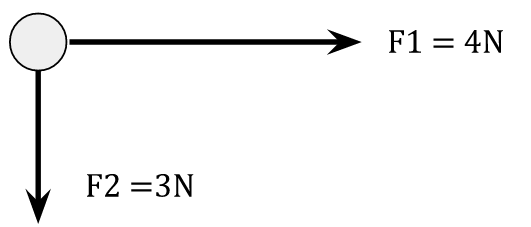
\includegraphics[width=20em]{kraft1}
            \end{center}

      \item
            \begin{minipage}[t]{0.6\textwidth}
                  En stege lutar mot en vägg, den väger 15
                  kg. Det finns en friktionskraft mellan stegen och marken
                  som är på 60 N.

                  Rita ut
                  och beräkna fler krafter som kan tänkas finnas för att
                  stegen ska vara i
                  jämvikt. \textbf{(3p)}
            \end{minipage}
            \hspace{2em}
            \begin{adjustbox}{valign=t}
                  \includesvg[width=10em]{stege}
            \end{adjustbox}

      \item
            En bro som väger 5 ton ligger på två stödytor och är i jämvikt.
            Avstånd mellan tyngdpunkt och vänster stödyta är 7 meter och
            avstånd mellan
            tyngdpunkt och höger stödyta är 3 meter.
            Beräkna hur mycket kraft varje stödyta tar upp. \textbf{(4p)}
            \begin{center}
                  \includesvg[width=0.8\textwidth]{bro}
            \end{center}

\end{enumerate}
\end{document}